\documentclass[twoside]{article}

% AISTATS 2027 submission format.
\usepackage[numbers,compress]{natbib}
\usepackage{aistats2027}

\usepackage[utf8]{inputenc}
\usepackage[T1]{fontenc}
\usepackage{graphicx}
\usepackage[percent]{overpic}
\graphicspath{{figures/}}
\usepackage{hyperref}
\hypersetup{
  colorlinks=true,
  linkcolor=black,
  citecolor=black,
  urlcolor=black,
  pdfborder={0 0 0}
}
\usepackage{url}
\usepackage{booktabs}
\usepackage{multirow}
\usepackage{amsfonts}
\usepackage{amsthm}
\usepackage{nicefrac}
\usepackage{microtype}
% \usepackage{xcolor}
\usepackage[dvipsnames]{xcolor}

\newcommand{\note}[1]{\colorbox{BurntOrange}{(#1)}}

\newtheorem{lemma}{Lemma}
\newtheorem{proposition}{Proposition}
\newtheorem{corollary}{Corollary}
\begin{document}

\twocolumn[
\aistatstitle{Determining Optimal Training Strategies Using Cross-Validation with Domains and Downsampling}
\aistatsauthor{Anonymous Author(s)}
\aistatsaddress{Anonymous Institution(s)}
]

\begin{abstract}
In many machine learning applications, data come with domains defined by geography, time period, acquisition protocol, demographic group, etc.
% Previous methods for estimating generalization error
When model performance differs across domains of different sizes, we would like to determine the cause (number of train data, or distributional difference between domains).
% If the gap reflects unequal training-set sizes, more data collection is needed; if it reflects genuine distributional differences, domain adaptation or robustness methods are needed.
% Standard cross-validation and the SOAK framework \citep{hocking2026} do not separate these two causes.
We propose SOKED (Same/Other K-fold cross-validation Extension: Downsampling), a new machine learning evaluation framework that formally decomposes an observed performance gap into a \emph{sample-size component} and a \emph{residual domain component} by using matched-size downsampling to equalize training set sizes.
% The decomposition can reverse the apparent ordering of training configurations: in our experiment on the dataset "workers' compensation", the naive full-data comparison suggests Other training data is superior, while SOKED shows the gap is not significant once training-set size is controlled.
After size matching, domain advantages either disappear (indicating a sample-size effect; domains are compatible), or persist (indicating a true distributional difference between domains), depending on the data set.
% , so domain adaptation methods may be required for optimal learning and prediction).
We show the advantages of the proposed SOKED framework relative to baselines, using simulations and real data sets from diverse domains: traffic monitoring, insurance claims, image classification, survey data, and microbial biogeochemistry.
% We implement SOKED in the \texttt{mlr3resampling} R package.
\end{abstract}


\section{Introduction}
In many real-world machine learning problems, the data fall into natural domains defined by time period, geographic region, collection protocol, demographic group, etc.
When model performance differs across these domains, it is not obvious whether the difference comes from genuine heterogeneity in the data or from the simpler fact that some domains contain more training examples than others.

For example, consider creating a public health monitoring system using data from the National Survey of Children’s Health \citep{NSCH2019}, which contains domains for different years of data collection (18,202 survey responses in 2019 and 27,808 in 2020).
In the previous SOAK evaluation framework \citep{hocking2026}, we fix a test domain (2020), then systematically compare models trained using data from either the same year (2020), or from the other year (2019).
If the model trained on the same year performs better than the model trained on the other year, is this improvement because there are more training examples (sample size effect), or because the other year has a different data distribution (domain effect) that makes learning and prediction more difficult?
% If the gain comes solely from the sheer data volume, then the practical response is to combine years when training.
If real distributional shifts exist between years, then separate models can be trained for each year, or data can be combined using domain adaptation techniques \citep{CostaJussa2015}.
However, the previous SOAK framework does not separate domain effects (distributional differences) from sample-size effects (performance gains due to more training data), so its conclusions can be misleading when domains differ substantially in size.

We propose SOKED (\textbf{S}ame/\textbf{O}ther \textbf{K}-fold cross-validation \textbf{E}xtension: \textbf{D}ownsampling), a new evaluation framework that formally decomposes an observed performance gap into a \emph{sample-size component} and a \emph{residual domain component}.
By holding training set size fixed through matched downsampling, SOKED empirically estimates the cause of performance differences: either a sample-size effect (the ordinary benefit of more training data) or a domain effect (genuine differences in learnable patterns between domains).
% The decomposition changes the recommended action: a sample-size effect calls for collecting more data, while a residual domain effect calls for distributional robustness methods or domain adaptation.

% The decomposition can also reverse the apparent ordering of training configurations and expose a failure mode of naive full-data comparison.
% In our experiment on the dataset "workers' compensation", the full-data comparison favors the Other model for female domain; after size-matching, SOKED shows the gap shrinks to non-significance ($p > 0.1$), revealing that the apparent advantage is largely explained by training-set size rather than a genuine distributional difference.
% We demonstrate this and related phenomena across simulated regression, benchmark classification (STL-10, Waveform), epidemiological survey data (NSCH autism), and microbial biogeochemistry (qSIP).

\textbf{Summary of contributions.}
We present three contributions.

\textbf{1. New SOKED evaluation framework, which fills an important practical gap in available machine learning open source software.}
  We propose SOKED, a new evaluation framework which uses downsampling to distinguish sample-size effects from residual domain effects.
  To our knowledge, no prior software implements this Same/Other diagnostic with matched-size comparisons, so SOKED fills a practical software gap for cross-validation over predefined domains.


\textbf{2. Mathematical analysis.}
  We introduce a decomposition of cross-validation performance gaps into a sample-size component and a residual domain component, using matched-size downsampling.
  Lemma~\ref{lem:exchangeability} gives a sufficient condition under which the domain component is zero.

\textbf{3. Benchmark file format and empirical demonstrations.}
  We propose a simple standard file format for benchmarking Same/Other domain comparisons and release eight datasets in that format.
  % Each benchmark file makes the resampling splits, domains, target, and predictors explicit using \texttt{fold}, \texttt{domain}, \texttt{y}, and \texttt{x} columns.
  We use these data to highlight the novelty of the proposed SOKED algorithm, which separates apparent advantages caused by unequal training-set sizes from residual domain effects that persist after size matching.


\section{Related work}

\textbf{Open source software for cross-validation.} K-fold cross-validation is a standard algorithm for model assessment \citep{stone1974cross,geisser1975predictive,Arl_Cel:2010:surveyCV}, which is implemented in modern machine learning frameworks such as \texttt{mlr3} in R and \texttt{scikit-learn} in Python \citep{Bischl2024,scikit-learn}.
Some packages support structured resampling methods, to account for imbalance, as well as spatial, temporal, or hierarchical dependencies, by using strata with blocking or grouping \citep{roberts2017,brenning2005,valavi2019,schratz2024}.
These mechanisms control how folds are formed; the proposed SOKED framework answers a different question: after the test domain is fixed, which domain(s) can be used for optimal training, and how much of any observed performance gap is due to different domain sizes, and how much is due to genuine distributional differences between domains?
%\textbf{Software.}
Whereas existing implementations of cross-validation such as scikit-learn support ``groups'' and ``strata,'' the proposed SOKED framework uses a new ``domain'' variable (Figure~\ref{fig:SOKED-concept}), for which there is not yet support in scikit-learn.

\begin{figure*}[!t]
    \centering
    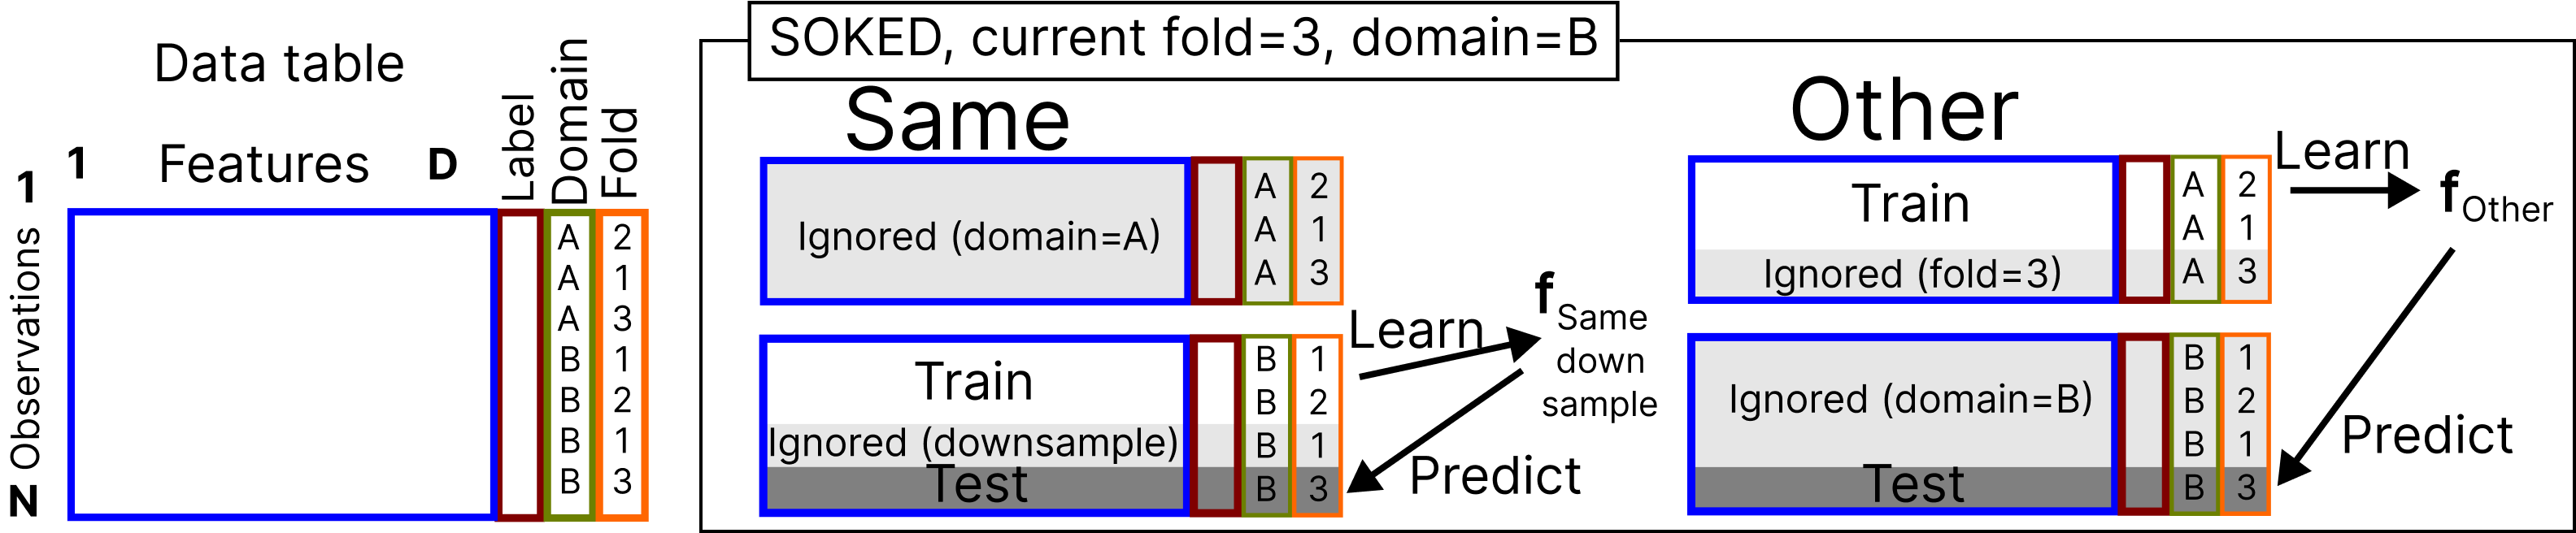
\includegraphics[width=0.9\textwidth]{fig1-concept-domain.png}
    \caption{
    Proposed SOKED evaluation framework (3-fold cross-validation), for test fold=3 and test domain=B, in data with two domains of different sizes: A has three rows and B has four rows.
    After excluding data based on fold and domain, random downsampling is used to obtain train sets of size equal to the smaller train set (Other, 2 rows).}
    \label{fig:SOKED-concept}
\end{figure*}
\textbf{Distribution shift and transfer learning.}
Transfer learning and domain adaptation methods are prescriptive: given a distributional shift, they adapt a source model to a target domain \citep{pan2010transfer,Farahani2021}.
The proposed SOKED framework is instead diagnostic: it determines whether same-domain or other-domain training data are more predictive for a fixed target domain, and decomposes any gap into a sample-size component and a residual domain component.
The previous SOAK framework includes a comparison with training on all domains, but does not include downsampling, so is not able to determine the cause of performance differences when training on domains of unequal sizes \citep{hocking2026}.
The proposed SOKED framework focuses on the Same/Other contrast and proposes a new downsampling method to handle the practically important case of unequal domain sizes.

\textbf{Fairness auditing.}
Demographic subgroups are often imbalanced in size, so an observed performance disparity may reflect either genuine distributional differences or simply less training data for the disadvantaged group \citep{savoldi2021gender,hall2024visogender}.
SOKED separates these two causes: a sample-size finding calls for targeted data collection, while a residual domain effect calls for bias mitigation strategies.



\section{Methods}


\subsection{Proposed SOKED evaluation framework}
\label{sec:workflow}
The goal of the proposed SOKED method is to determine if data domains of different sizes are similar enough for optimal learning and prediction.
The steps of SOKED are:
% We fix a test fold and a target domain, then compare predictors trained on either the Same domain, or the Other domain.
% SOKED retains both the original full-data training sets and matched-size versions obtained by random downsampling to the smaller feasible training set, so the full-data gap and the size-controlled gap can be compared.
% For one target domain, SOKED proceeds as follows.
\begin{enumerate}
    \item \textbf{Fix the test domain.} Choose the target domain whose test performance will be evaluated.
    As shown in Figure~\ref{fig:SOKED-concept}, the test set is defined as the intersection of the current fold and domain.
    \item \textbf{Analyze full train size results.}
    Define the full train set as all of the data in the Same or Other domain, except the data in the current fold (which is either ignored or used as test set).
    Compute prediction error for Same and Other models and K-fold CV.
    Use Table~\ref{tab:scenario-interpretation} to interpret the p-value for test error differences between Same and Other.
    If the model trained on the larger domain is more accurate (scenarios S or O), then proceed to step 3.
    Otherwise, there must be a domain effect (scenarios C and D, some difference between domains).
    \item \textbf{Analyze matched size results.}
    Compute prediction error for Same and Other models, after downsampling the larger of the two training sets to the smaller size.
    A significant p-value for difference between Same/Other test error rates is evidence for a domain effect.
    Otherwise, a p-value that is no longer significant after matching is evidence of a sample size effect (domains are consistent for learning and prediction).
\end{enumerate}
Table~\ref{tab:scenario-interpretation} summarizes the qualitative interpretation of Same against Other at Step 2 (before downsampling).
When the smaller source already performs better (Scenarios C and D), that is immediate evidence of a domain effect (some difference between domains exists, so no need to perform downsample analysis).
When the larger source also performs better (Scenarios S and O), the result is ambiguous under unequal training sizes, so SOKED proceeds to downsample analysis in step 3.
% Figure~\ref{fig:SOKED-concept} summarizes the SOKED step 3, for one  cross-validation fold and one target domain.

\begin{table*}[!t]
\centering
\small
\caption{Interpretation of predictive performance and sample size at Step 2 of the proposed SOKED evaluation framework.}
\label{tab:scenario-interpretation}
\begin{tabular}{p{0.22\textwidth} p{0.34\textwidth} p{0.34\textwidth}}
\toprule
\textbf{Sample size} & \textbf{Other better than Same} & \textbf{Same better than Other} \\
\midrule
\textbf{Other larger than Same}
& Why is Other better?
\newline $\bullet$\ Is it a sample size effect?
\newline $\bullet$\ Or a domain effect?
\newline \textbf{Scenario O}
& It must be a domain effect. \textbf{Domains are too different} for optimal learning and prediction.
\newline \textbf{Scenario D} \\
\addlinespace
\textbf{Same larger than Other}
& It must be a domain effect. Other is a \textbf{consistent pattern} with less noise that is easier to learn.
\newline \textbf{Scenario C}
& Why is Same better?
\newline $\bullet$\ Is it a sample size effect?
\newline $\bullet$\ Or a domain effect?
\newline \textbf{Scenario S} \\
\bottomrule
\end{tabular}
\end{table*}


\subsection{Operational decomposition of performance gaps}
Consider two training configurations $a,b \in \mathcal C$, where typically
$\mathcal C=\{\mathrm{Same},\mathrm{Other}\}$.
Let $L(\hat f_{c,n})$ denote the test loss on target domain of a predictor trained under configuration $c$ using $n$ training examples, where lower values indicate better performance.
Throughout, we express performance as a loss with lower values indicating better performance in our experiments.
We average test losses over outer cross-validation folds.

Let $n_a$ and $n_b$ denote the full available training sizes for configurations $a$ and $b$, respectively, and let $n_0 = \min(n_a,n_b)$ denote the matched training size used after downsampling.
We compare the full-data and matched-size gaps:
\begin{equation}
\begin{aligned}
\Delta^{\mathrm{full}}
&:= L(\hat f_{a,n_a}) - L(\hat f_{b,n_b}), \\
\Delta^{\mathrm{match}}
&:= L(\hat f_{a,n_0}) - L(\hat f_{b,n_0}).
\end{aligned}
\label{eq:gaps}
\end{equation}


\textbf{Why match at the minimum size?}
SOKED answers the question: \emph{would the larger-domain configuration still win if it only had as much data as its competitor?}
If not, the observed advantage is fully explained by sample size.
This is an operational decomposition: the matched-size gap is interpreted as the residual domain component after controlling for training size, and the difference between the full-data and matched-size gaps is attributed to unequal training size.
The domain component should be interpreted broadly as the residual performance difference at matched training size.
This residual may reflect source-target alignment, label noise, class balance, or other factors affecting the usefulness of samples for the target task.
The following result gives a formal condition under which the domain component is zero, providing an anchor for the decomposition.

\begin{lemma}[Exchangeability implies zero matched-size gap]
\label{lem:exchangeability}
Suppose domains $a$ and $b$ are i.i.d.\ from the same marginal distribution $P_{X,Y}$, and that the learner is symmetric in its training examples.
Then $\mathbb{E}[\Delta^{\mathrm{match}}] = 0$ for all matched training sizes $n_0$.
Consequently, a persistent nonzero empirical matched-size gap is evidence against exchangeability of the two domains, subject to sampling variability.
\end{lemma}

The same decomposition explains ordering reversals: one configuration can be better at matched size, while another can win in the full-data comparison only because it has more training examples.
% Appendix~\ref{app:proofs} gives a formal characterization.


\subsection{Statistical test for the domain effect}
\label{sec:ttest}
Lemma~\ref{lem:exchangeability} establishes that $\mathbb{E}[\Delta^{\mathrm{match}}] = 0$ when the two domains are exchangeable, making the matched-size gap a natural test statistic for a genuine domain effect.
We test $H_0\colon \mathbb{E}[\Delta^{\mathrm{match}}] = 0$ using a paired $t$-test on fold-level gap estimates.

We compute the matched-size loss difference for differences within each fold from $1$ to $K$.
We then apply a paired $t$-test to $\{\Delta_1^{\mathrm{match}},\ldots,\Delta_K^{\mathrm{match}}\}$ against the null mean of zero.
Rejecting $H_0$ is evidence of a domain effect that the sample-size component alone cannot explain.


\begin{table*}[t]
\centering
\scriptsize
\setlength{\tabcolsep}{2pt}
\caption{Summary of data sets used in the experiments. Note: Imb.\ = imbalance ratio between domains (1 = balanced; larger values indicate more imbalance).}
\label{tab:dataset-summary}
\begin{tabular}{p{0.13\linewidth}p{0.32\linewidth}rrrp{0.16\linewidth}l}
\toprule
\textbf{Dataset} & \textbf{Domain names and sizes} & \textbf{Rows} & \textbf{Feature(s)} & \textbf{Domain imb.} & \textbf{Target} & \textbf{Task} \\
\midrule
Different & large(400) / small(200) & 600 & 1 & 2.00 & y & Regression \\
IID easy & large(80) / small(40) & 120 & 1 & 2.00 & y & Regression \\
\midrule
qSIP &  qme.15(4,590) / dim.control(3,120) & 7,710 & 8,380 & 1.47 & growth\_per\_day & Regression \\
Traffic & Phoenix(110,414) / Baltimore(18,378) & 128,792 & 7 & 6.01 & log(AADT) & Regression \\
Workers' comp & Male(77,172) / Female(22,828) & 100,000 & 8 & 3.38 & log(claim cost) & Regression \\
\midrule
NSCH autism & 2020(27,808) / 2019(18,202) & 46,010 & 362 & 1.53 & Autism diagnosis & Classification \\
STL-10 & test(8,000) / train(5,000) & 13,000 & 27,648 & 1.60 & Image class & Classification \\
Waveform & test(500) / train(300) & 800 & 21 & 1.67 & Waveform class & Classification \\
\bottomrule
\end{tabular}
\end{table*}

\section{Data sets and empirical results}
\label{sec:experiments-results}
\subsection{Experimental setup}
\label{sec:datasets}
Our goal in this section is to show a variety of data sets, in which the proposed SOKED framework leads to different conclusions about the similarity of domains.
In particular, we aim to emphasize situations where the previous SOAK framework \citep{hocking2026} (full train set size/no downsampling) is not sufficient, and the proposed downsampling is necessary to obtain an accurate interpretation about which domains have similar or different patterns for learning and prediction.
We therefore applied SOKED to two simulated and six real datasets that span regression and classification, low and high-dimensional features, and natural domain structures defined by geography, time, treatment, demography, and benchmark splits.
Table~\ref{tab:dataset-summary} summarizes their key properties.
All experiments use 10-fold cross-validation and report classification error rate or RMSE.
Each data set has two domains.
We show detailed results for some illustrative test domains in Figures 2--5, and we show a summary of results for all test domains in Table~\ref{tab:results-summary}.
Experiments were conducted on a SLURM HPC cluster, with individual jobs requiring less than two hours of wall-clock time and approximately 16\,GB of memory.


\textbf{Proposed benchmark file format.}
We publish each data set as a CSV file with rows for data observations and named columns ordered as follows: first column named \texttt{fold} contains a randomly assigned integer fold ID, second column named \texttt{subset} stores the domain label (the field name is retained for software compatibility), third column named \texttt{y} contains output to predict, and other columns are inputs for prediction.
% The proposed SOKED framework compares predictive performance when training on Same and Other domains.
% It directly tests whether domain identity matters after controlling for training size.
% \paragraph{Data availability and licensing.}
% All datasets used in this paper are publicly available.
% STL-10 \citep{coates2011stl10} and the UCI Waveform dataset \citep{breiman1984classification} are distributed under their original public-research licenses.
% NSCH micro-data are released by the U.S.\ Census Bureau and the Health Resources and Services Administration for public research use.
% The workers' compensation dataset is a synthetic benchmark released with \citet{Ali2020}.
% The traffic and qSIP datasets were produced by collaborating research groups and are made available with the SOKED code release.
% Preprocessing scripts and the exact dataset versions used in our experiments are included with the accompanying \texttt{mlr3resampling} code release to support full reproducibility.
% TODO

\subsection{Simulated regression data sets}
The simulations were chosen to illustrate cases in which there is clearly either a sample size effect (\texttt{iid\_easy}), or a domain effect (\texttt{different}), using a simple decision tree learner (rpart in mlr3 with default settings).
Both data sets involve one feature $x\sim U[-3\pi,3\pi]$ (uniform distribution), with $y=\sin(x)+\epsilon$, and $\epsilon\sim N(0, \sigma^2)$.
In \texttt{iid\_easy} data, both large (80 samples) and small (40 samples) domains are i.i.d. with $\sigma=0.1$, so any full-data gap should disappear after size-matching (sample size effect, Lemma~\ref{lem:exchangeability}).
In \texttt{different}, the large domain (400 samples) has less noise ($\sigma=0.1$) than the small domain ($\sigma=1.7$), so a Same--Other gap reflects a genuine domain effect (test error difference should stay after size matching).
% Both are used to assess seed robustness with 100 independent downsampling seeds and to verify that SOKED recovers the expected distinction between true domain differences and pure size imbalance.
% In Figure~\ref{fig:sim-combined}, we assess whether the SOKED conclusion is stable across random downsampling seeds.
We repeated the proposed SOKED procedure with 100 independent random seeds and examined the distribution of paired $t$-test $p$-values across seeds (Figure~\ref{fig:sim-combined}).
% The blue vertical line gives the $p$-value using the full (unequal size) training sets; the red boxplots summarize the distribution of $p$-values across the 100 downsampling seeds.

For \texttt{different} (top row), all 100 downsampled $p$-values are well below $0.05$ for both test domains, confirming that the domain effect is detected robustly, regardless of which random seed is used.
For \texttt{iid\_easy} (bottom row), the full-data test error difference is significant (blue line left of the threshold), but after downsampling, differences are no longer significant ($p > 0.01$).
This confirms that the full-data signal is driven by the sample-size imbalance and disappears once training sizes are equalized, consistent with Lemma~\ref{lem:exchangeability}.
The robustness of these conclusions across 100 seeds supports the practical use of a single seed especially in situations where compute is limited.

\begin{figure*}[!t]
    \centering
    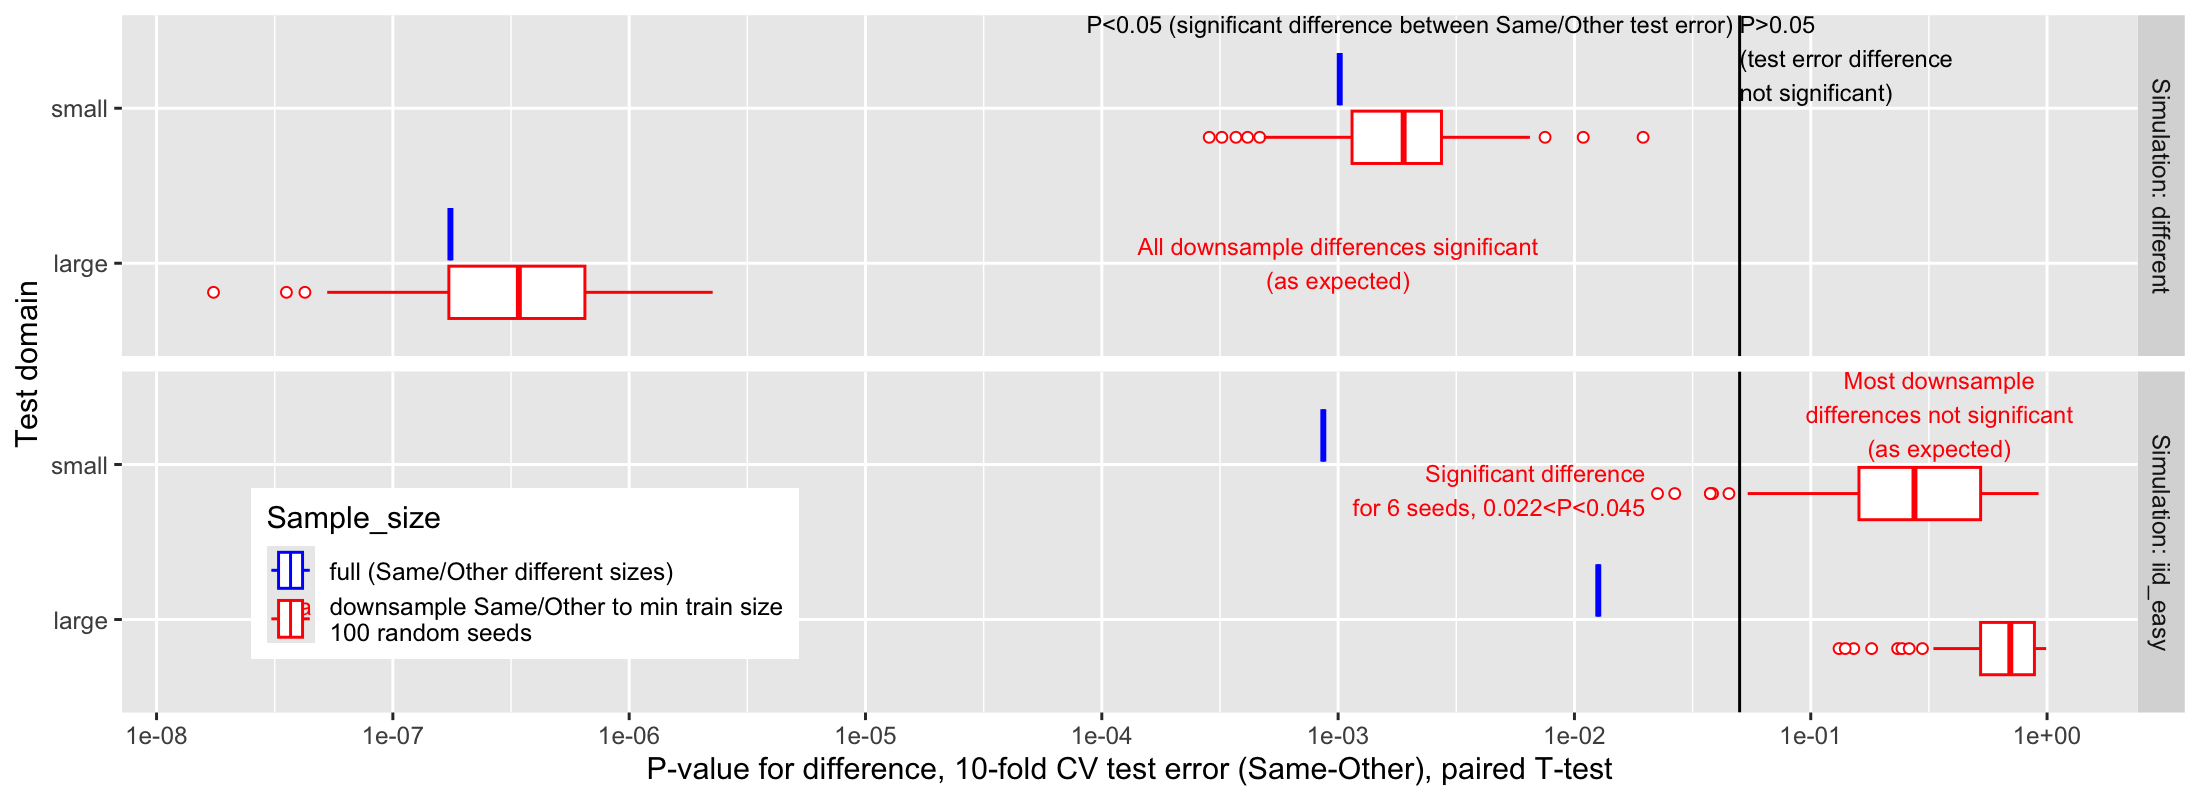
\includegraphics[width=0.95\textwidth]{fig3-simulations-domain.png}
    \caption{Robustness of proposed SOKED evaluation framework, over 100 downsampling seeds in simulations (\texttt{different} and \texttt{iid\_easy}), using the rpart learner. Blue shows the full-data Same--Other p-value; red boxes show matched-size p-values across seeds.}
    \label{fig:sim-combined}
\end{figure*}

\subsection{Real regression data sets}
We next consider the three real regression examples, beginning with the traffic data because it motivates the learner choice used in the remaining regression experiments.

\textbf{Traffic.}
In these data, we want to determine if models for predicting traffic (and on-road carbon emissions) can generalize between two different cities (Phoenix and Baltimore, which are the two SOKED domains).
The traffic dataset contains gapfilled \citep{Gurney2025Vulcan} road-segment observations from the Highway Performance Monitoring System \citep{FHWA2016HPMSShapefile}.
Each row represents one road segment, the prediction target is log-transformed Average Annual Daily Traffic (AADT) \citep{bilal_hpms_aadt}, and the feature set combines night-time lights \citep{bilal_ntl_viirs}, population \citep{bilal_worldpop}, road density \citep{bilal_osm_roads}, and Sentinel-2 \citep{bilal_sentinel2} satellite bands.
The Sentinel-2 bands are RGB and NIR (red, green, blue, and near-infrared).

% We also use this dataset to assess learner robustness, comparing featureless, \texttt{rpart}, \texttt{glmnet}, and a torch-based MLP over 5-fold CV.
We assess whether the SOKED conclusion depends strongly on the prediction algorithm by using 5-fold CV to compare several learners: constant baseline (featureless), regression tree (\texttt{rpart}), L1-regularized linear model (\texttt{glmnet}), and a multi-layer perceptron (MLP).
These learners span increasing model flexibility and complexity.
The featureless learner predicts the training-set mean and serves as a no-signal baseline in \texttt{mlr3} \citep{Bischl2024}.
\texttt{rpart} is the default decision tree learner for regression in the mlr3 framework \citep{Breiman1984}.
\texttt{glmnet} fits a linear model with degree of L1 regularization chosen using internal 10-fold CV \citep{Friedman2010glmnet}.
The MLP for regression consists of two fully connected hidden layers with 32 and 16 neurons, respectively, and ReLU activation functions between layers.
The network was trained using the AdamW optimizer with a batch size of 16{,}384 and a Smooth L1 (Huber) loss function \citep{rtorch}.
Learning rates were selected based on validation performance with early stopping.
Figure~\ref{fig:learner-panels} focuses on the Phoenix test domain and reports test RMSE for the Same and Other train-domain configurations.

\begin{figure*}[!t]
    \centering
    \begin{overpic}[height=0.17\textheight,keepaspectratio]{fig2-learner-panels.png}
      \put(97.55,4){\color[gray]{0.85}\rule{1.7\unitlength}{19.4\unitlength}}
      \put(98.3,13.7){\rotatebox{270}{\makebox(0,0){\sffamily\fontsize{6}{7}\selectfont Test domain: Phoenix}}}
    \end{overpic}
    \caption{SOKED for four learning algorithms on traffic data (Phoenix test domain), comparing training on Same and Other domains, at full and matched training sizes.}
    \label{fig:learner-panels}
\end{figure*}


Figure~\ref{fig:learner-panels} shows that training on the Same domain is consistently better than training on the Other domain, even after train-size matching.
All learners we see consistent Same/Other error rate differences using full and downsampled train sizes, which implies a clear domain effect (some distributional difference between cities, that sample size alone can not explain).
The smallest RMSE comes from the MLP, followed by \texttt{glmnet} and then \texttt{rpart}.
Interestingly, the Other models for \texttt{rpart} and \texttt{MLP} learners have larger error rates than the featureless baseline, which implies that the cities are too different for these algorithms to learn any kind of useful predictions across cities.
The Other model for \texttt{glmnet} has slightly smaller error than featureless, which implies that the linear model is able to learn something non-trivial, although it is not nearly as accurate as the Same model.
Overall, these results on the traffic data highlight how the SOKED conclusions depend on the learning algorithm as well as the data set.

\textbf{qSIP.}
The qSIP dataset comes from quantitative stable isotope probing experiments \citep{hungate2015quantitative}, performed in various sites and time periods.
We would like to determine if the control samples have learnable/predictable patterns that generalize between experiments.
Controls were combined from two experiments (DIM and QME), yielding data with two domains: \texttt{dim.control} (3,120 samples) and \texttt{qme.15} (4,590 samples).
Each row is an observation characterized by 8,380 KEGG ortholog indicators, and the prediction target is \texttt{growth\_per\_day}.
If our goal is to predict growth rate for \texttt{qme.15}, we would like to know whether training on \texttt{qme.15} is more accurate than training on \texttt{dim.control} because QME has more examples, or because the two experiments have different learnable growth patterns.

For qSIP, Figure~\ref{fig:regr-pairs} (middle column) shows SOKED results for the \texttt{qme.15} test domain.
At full training sizes, Same ($N = 4{,}131$) outperforms Other ($N = 2{,}808$), so the naive comparison could be attributed to Same having more training examples.
After downsampling Same to $n_0 = 2{,}808$, the gap still persists with $p < 0.001$, confirming a strong domain effect.
The conclusion is that the two experiments/domains are too different for the rpart algorithm to do accurate learning and prediction.

\textbf{Workers' compensation.}
The workers' compensation dataset is a benchmark of 100,000 synthetically generated insurance claims \citep{Ali2020}.
Each row represents one claim, the prediction target is log-transformed UltimateIncurredClaimCost, and claimant gender defines the two SOKED domains: 77,020 males and 22,980 females.
If our goal is to have good predictions for females, we would like to know if training on males is more accurate because of the increased sample size.

For workers' compensation, Figure~\ref{fig:regr-pairs} (right column) shows the Female test domain.
At full training sizes, Other ($N = 69{,}454$) outperforms Same ($N = 20{,}545$) in RMSE.
After downsampling to $n_0 = 20{,}545$, the gap  is no longer significant ($p = 0.117$).
This is the sample-size pattern SOKED is designed to reveal.
Most of the apparent full-data advantage of Other is explained by its larger training set size.
The conclusion from SOKED is that male and female domains in these data are consistent enough for accurate learning and prediction using the rpart decision tree algorithm.

\begin{figure*}[!t]
    \centering
    \def\pairfigure{fig5-regr-pairs.png}
    \def\firstdomain{Phoenix}\def\seconddomain{qme.15}\def\thirddomain{F}
    % Preserve the numerical plot and replace only its domain labels.
\begin{overpic}[height=0.17\textheight,keepaspectratio]{\pairfigure}
  \put(0,7){\color{white}\rule{2.2\unitlength}{12\unitlength}}
  \put(1.2,12.9){\rotatebox{90}{\makebox(0,0){\sffamily\fontsize{7}{8}\selectfont Train domains}}}
  \put(10.3,21.35){\color[gray]{0.85}\rule{27.2\unitlength}{1.7\unitlength}}
  \put(38.6,21.35){\color[gray]{0.85}\rule{27.2\unitlength}{1.7\unitlength}}
  \put(66.95,21.35){\color[gray]{0.85}\rule{27.2\unitlength}{1.7\unitlength}}
  \put(23.9,22.25){\makebox(0,0){\sffamily\fontsize{6.5}{7}\selectfont Test domain: \firstdomain}}
  \put(52.2,22.25){\makebox(0,0){\sffamily\fontsize{6.5}{7}\selectfont Test domain: \seconddomain}}
  \put(80.6,22.25){\makebox(0,0){\sffamily\fontsize{6.5}{7}\selectfont Test domain: \thirddomain}}
\end{overpic}

    \caption{
    SOKED results for three regression datasets (rpart learner, 10-fold CV), comparing Same and Other at full and matched training sizes by target domain.
    Each column corresponds to one dataset/test-domain pair.}
    \label{fig:regr-pairs}
\end{figure*}


\subsection{Real classification data sets}
We analyzed three real classification data sets, using the \texttt{glmnet} regularized linear model.
The data sets were chosen to show how the proposed SOKED analysis leads to different conclusions, depending on the data distribution.

\textbf{NSCH autism.}
The National Survey of Children's Health (NSCH) is a nationally representative annual survey conducted by the U.S.\ Census Bureau \citep{NSCH2019,NSCH2020}.
We use survey years 2019 and 2020 as the two SOKED domains (18,202 and 27,808 children, respectively).
Each row represents one child ages 3-17 years, with survey responses provided by an adult familiar with the child's health, and the features encode questionnaire items on condition diagnoses, family income, insurance coverage, healthcare access, neighborhood conditions, and other health-related factors.
The target is a binary autism identification (was the child ever diagnosed with autism by a doctor/other healthcare provider) indicator.
If our goal is to have good predictions for 2020, we would like to know if training on 2020 is more accurate because of the increased sample size, or because it is somehow different from 2019.

Figure~\ref{fig:classif-pairs} (left column) shows SOKED results for the 2020 test domain.
The full-data comparison favors Same ($N=25{,}027$) over Other ($N=16{,}381$), and the gap is significant ($p < 0.01$).
After downsampling to $n_0 = 16{,}381$, the gap narrows but does not disappear.
Same still has lower error than Other, and the matched-size gap still remains significant ($p \approx 0.01$).
This indicates a modest residual year-specific domain effect in addition to the sample-size advantage.
For the 2019 test domain, the pattern is different.
Other is better at full size because it has more data, but the matched-size gap is non-significant ($p > 0.1$), which is consistent with a sample-size effect.
Taken together, NSCH shows both effects across years.
Predicting on 2020 shows a small residual domain effect, whereas predicting on 2019 shows a sample size effect.
Taken together, these results suggest that years in these survey data are mostly consistent, with some small differences that can affect prediction accuracy.

\textbf{STL-10.}
STL-10 is a benchmark image classification dataset \citep{coates2011stl10} with 13,000 images, each with 96x96 pixels in 3 color channels (27,648 features), across 10 object classes.
Each row is one image, the target is object class, and the predefined train (5,000) and test (8,000) splits serve as the two SOKED domains.
If our goal is to have good predictions on a held-out set of images drawn from the test domain, we would like to know if learning using the other images from the test domain is as accurate as learning using images from the train domain.

Figure~\ref{fig:classif-pairs} (middle column) shows SOKED results when predicting on the predefined test domain.
At full training sizes, Same ($N=7{,}200$) outperforms Other ($N=4{,}500$), and the gap is significant ($p < 0.001$).
After downsampling to $n_0 = 4{,}500$, the gap narrows and becomes non-significant ($p > 0.1$), consistent with a sample-size effect.
When the predefined train domain is the prediction target, Other is better at full size, but the matched-size gap is also non-significant ($p > 0.1$), again consistent with a sample-size effect.
These data indicate that the predefined train/test domains in STL-10 data are consistent with random division of the data (and no distributional difference between predefined train/test sets, at least for the glmnet learner).

\textbf{Waveform.}
The UCI Waveform dataset \citep{Breiman1984} contains 800 labeled examples (300 train, 500 test) across three classes described by 21 features after preprocessing.
Each row is one waveform example, the target is waveform class, and the predefined train/test split defines the two SOKED domains.
Our goal is to determine whether or not data have a consistent pattern across the predefined train/test split.

Figure~\ref{fig:classif-pairs} (right column) shows SOKED results when predicting on data from the predefined train domain.
At full training sizes, Other ($N=450$) outperforms Same ($N=270$), with a modest but significant gap ($p < 0.05$).
After downsampling to $n_0 = 270$, the gap narrows substantially.
Other error rate increases, and the matched-size comparison is non-significant ($p > 0.1$).
For this target domain, the apparent advantage of training on the Other domain is therefore largely explained by its larger training size rather than by a strong residual domain effect.
When the test split is the target, there is no significant difference between Same/Other at full train size ($p=0.598$), so we can immediately conclude that domains are similar.
We therefore stop at Step 2 of SOKED, and there is no need for Step 3 (downsampling/size-matching would not change our conclusions).
Taken together, SOKED indicates that Same/Other differences in Waveform data are explained by a sample size effect, which implies that the predefined train/test domains are consistent for learning using the glmnet algorithm.

\begin{figure*}[!t]
    \centering
    \def\pairfigure{fig4-classif-pairs.png}
    \def\firstdomain{2020}\def\seconddomain{test}\def\thirddomain{train}
    % Preserve the numerical plot and replace only its domain labels.
\begin{overpic}[height=0.17\textheight,keepaspectratio]{\pairfigure}
  \put(0,7){\color{white}\rule{2.2\unitlength}{12\unitlength}}
  \put(1.2,12.9){\rotatebox{90}{\makebox(0,0){\sffamily\fontsize{7}{8}\selectfont Train domains}}}
  \put(10.3,21.35){\color[gray]{0.85}\rule{27.2\unitlength}{1.7\unitlength}}
  \put(38.6,21.35){\color[gray]{0.85}\rule{27.2\unitlength}{1.7\unitlength}}
  \put(66.95,21.35){\color[gray]{0.85}\rule{27.2\unitlength}{1.7\unitlength}}
  \put(23.9,22.25){\makebox(0,0){\sffamily\fontsize{6.5}{7}\selectfont Test domain: \firstdomain}}
  \put(52.2,22.25){\makebox(0,0){\sffamily\fontsize{6.5}{7}\selectfont Test domain: \seconddomain}}
  \put(80.6,22.25){\makebox(0,0){\sffamily\fontsize{6.5}{7}\selectfont Test domain: \thirddomain}}
\end{overpic}

    \caption{
    SOKED results for three classification datasets (glmnet learner, 10-fold CV), comparing Same and Other at full and matched training sizes by target domain.
    Each column corresponds to one dataset/test-domain pair.}
    \label{fig:classif-pairs}
\end{figure*}


\begin{table*}[!t]
    \centering
    \small
    \resizebox{\linewidth}{!}{%
    \begin{tabular}{lllcccll}
\toprule
Data &  Test domain & Algorithm & Better (Full) & Larger & Scenario & Better (Matched) & Effect \\
\midrule
iid\_easy & small & rpart & other ($p = 0.016$) & other & O & equal ($p = 0.157$) & sample size \\
iid\_easy & large & rpart & same ($p = 0.019$) & same & S & equal ($p = 0.672$) & sample size  \\
different & small & rpart & other ($p = 0.002$) & other & O & other ($p = 0.002$) & domain \\
different & large & rpart & same ($p < 0.001$) & same & S & same ($p < 0.001$) & domain  \\
% \midrule
qSIP & qme.15 & rpart & same ($p < 0.001$) & same & S & same ($p < 0.001$) & domain \\
qSIP & dim.control & rpart & other ($p < 0.001$) & other & O & other ($p < 0.001$) & domain \\
workers' comp & Male & rpart & same ($p < 0.001$) & same & S & same ($p < 0.001$) & domain \\
workers' comp & Female & rpart & other ($p < 0.001$) & other & O & equal ($p = 0.117$) & sample size \\
traffic & Phoenix & rpart & same ($p < 0.001$) & same & S & same ($p < 0.001$) & domain \\
traffic & Baltimore & rpart & other ($p < 0.001$) & other & O & other ($p < 0.001$) & domain \\
% \midrule
NSCH\_autism & 2019 & glmnet & other ($p = 0.030$) & other & O & equal ($p = 0.755$) & sample size \\
NSCH\_autism & 2020 & glmnet & same ($p = 0.004$) & same & S & same ($p = 0.013$) & domain \\
STL-10 & test & glmnet & same ($p < 0.001$) & same & S & equal ($p = 0.193$) & sample size \\
STL-10 & train & glmnet & other ($p < 0.010$) & other & O & equal ($p = 0.070$) & sample size \\
Waveform & test & glmnet & equal ($p = 0.598$) & same & - & - & similar  \\
Waveform & train & glmnet & other ($p = 0.046$) & other & O & equal ($p = 0.533$) & sample size \\
\bottomrule
\end{tabular}}
    \caption{SOKED results across all datasets.
    }
    \label{tab:results-summary}
\end{table*}

\subsection{Summary of results across all data sets}
Table~\ref{tab:results-summary} consolidates the dataset findings into a single view that reports which source performs better before and after matching, along with which source is larger.
These are the explanations for the scenario codes: O means Other is larger and also wins before matching, S means Same is larger and also wins before matching.
The Better(Full) and Better(Matched) columns show which model is better, along with P-values for Same/Other test error differences.
In one test domain, a dash (\emph{-}) means matching is not needed for interpretation (full train size results already indicate domain similarity in waveform test).
Of the 16 dataset/test-domain rows, 8 yield a residual domain effect that survives downsampling, and 7 collapse to a sample-size effect, illustrating that both regimes occur in practice rather than one dominating.
The O and S rows are the ones that the proposed SOKED framework is needed to resolve.
They are exactly the cases where the larger source could be winning either because it is larger or because it is genuinely more predictive.
If the previous SOAK method \cite{hocking2026} was used (no downsampling), then we would falsely conclude there is a distributional difference between domains, when in fact there is only a sample size effect, in 7 test domains.


\section{Conclusion}
SOKED extends Same/Other cross-validation with matched-size downsampling to separate a sample-size component from a residual domain component. Comparing full and matched training sizes helps distinguish settings where more data may help from those warranting distributional robustness or domain adaptation.

Across six real and two simulated datasets, both sample-size and residual domain effects occur (Table~\ref{tab:results-summary}). The simulations assess stability across 100 downsampling seeds, while the traffic experiment shows that the Same-beats-Other conclusion holds across different learners, with higher training costs for more expressive models.


SOKED is implemented in new open source software packages, in R and Python (URLs hidden during peer review).
Experiments and results can be found in this anonymous repository: \url{https://anonymous.4open.science/r/SOAKED-8FF7/}.
Future work includes extending the downsampling strategy to pooled training configurations to further isolate complementarity effects, and developing power analysis tools to guide the choice of number of folds and downsampling seeds.

\paragraph{Limitations.}
The decomposition is operational rather than causal: a persistent matched-size gap is evidence against exchangeability but does not identify which distributional factor drives it.
SOKED always matches at the minimum training size, the most conservative choice; when one domain is very large, this discards substantial data and reduces statistical power.
Finally, SOKED inherits the computational cost of running benchmark experiments at two training sizes; for expensive learners such as deep neural networks, this may be prohibitive.

\paragraph{Licensing and sensitive data.}
The released SOKED code and repository materials are available under the MIT License.
The NSCH data are de-identified public-use survey data, and the released benchmark files contain no personally identifiable information.

\section*{AI Use Statement}
Generative AI tools were used to edit the manuscript for grammar, spelling, terminology, and formatting, including figure labels and table layout.
They were not used to design the study, generate or analyze results, create the underlying plots, or establish mathematical claims.
The authors reviewed all AI-assisted edits and take responsibility for the final content.

\bibliographystyle{abbrvnat}
\bibliography{refs}

% \begin{proposition}[Characterization of ordering reversal]
% \label{prop:reversal}
% Let $f_c(n) = \mathbb{E}[L_t(\hat{h}_{c,n})]$ and suppose $n_b \geq n_a$, so $n_0 = n_a$.
% Let $\delta_q := f_b(n_0) - f_a(n_0)$ be the quality advantage of $a$ at matched size, and $\delta_s := f_b(n_0) - f_b(n_b) \geq 0$ be the size gain of $b$.
% Then $\mathbb{E}[\Delta_t^{\mathrm{match}}] = -\delta_q$ and $\mathbb{E}[\Delta_t^{\mathrm{full}}] = \delta_s - \delta_q$.
% Ordering reversal occurs if and only if $0 < \delta_q < \delta_s$: $a$ is the better source at matched size, but $b$'s size advantage is large enough to overcome that quality deficit.
% If $\delta_s = 0$, reversal is impossible and SOAK suffices; if $\delta_q = 0$, the gap is a pure sample-size effect.
% \end{proposition}

% \begin{proof}[Proof of Proposition~\ref{prop:reversal}]
% By definition, $\mathbb{E}[\Delta_t^{\mathrm{match}}(a,b)] = f_a(n_0) - f_b(n_0) = -\delta_q$.
% For the full-data gap, $\mathbb{E}[\Delta_t^{\mathrm{full}}(a,b)] = f_a(n_a) - f_b(n_b) = f_a(n_0) - f_b(n_b)$ (since $n_a = n_0$).
% Adding and subtracting $f_b(n_0)$ gives $f_a(n_0) - f_b(n_0) + f_b(n_0) - f_b(n_b) = -\delta_q + \delta_s = \delta_s - \delta_q$.
% Ordering reversal requires $\Delta_t^{\mathrm{match}}$ and $\Delta_t^{\mathrm{full}}$ to have opposite signs, i.e., $(-\delta_q)(\delta_s - \delta_q) < 0$, which holds iff $0 < \delta_q < \delta_s$.
% \end{proof}

\section*{Checklist}


\begin{enumerate}

  \item For all models and algorithms presented, check if you include:
  \begin{enumerate}
    \item A clear description of the mathematical setting, assumptions, algorithm, and/or model. [Yes]
    \item An analysis of the properties and complexity (time, space, sample size) of any algorithm. [No]
    \item (Optional) Anonymized source code, with specification of all dependencies, including external libraries. [Yes]
  \end{enumerate}

  \item For any theoretical claim, check if you include:
  \begin{enumerate}
    \item Statements of the full set of assumptions of all theoretical results. [Yes]
    \item Complete proofs of all theoretical results. [No]
    \item Clear explanations of any assumptions. [Yes]
  \end{enumerate}

  \item For all figures and tables that present empirical results, check if you include:
  \begin{enumerate}
    \item The code, data, and instructions needed to reproduce the main experimental results (either in the supplemental material or as a URL). [Yes]
    \item All the training details (e.g., data splits, hyperparameters, how they were chosen). [Yes]
    \item A clear definition of the specific measure or statistics and error bars (e.g., with respect to the random seed after running experiments multiple times). [Yes]
    \item A description of the computing infrastructure used. (e.g., type of GPUs, internal cluster, or cloud provider). [Yes]
  \end{enumerate}

  \item If you are using existing assets (e.g., code, data, models) or curating/releasing new assets, check if you include:
  \begin{enumerate}
    \item Citations of the creator If your work uses existing assets. [Yes]
    \item The license information of the assets, if applicable. [Yes]
    \item New assets either in the supplemental material or as a URL, if applicable. [Yes]
    \item Information about consent from data providers/curators. [Not Applicable]
    \item Discussion of sensible content if applicable, e.g., personally identifiable information or offensive content. [Yes]
  \end{enumerate}

  \item If you used crowdsourcing or conducted research with human subjects, check if you include:
  \begin{enumerate}
    \item The full text of instructions given to participants and screenshots. [Not Applicable]
    \item Descriptions of potential participant risks, with links to Institutional Review Board (IRB) approvals if applicable. [Not Applicable]
    \item The estimated hourly wage paid to participants and the total amount spent on participant compensation. [Not Applicable]
  \end{enumerate}

\end{enumerate}


\end{document}
